\documentclass[tikz]{standalone}
\usepackage{tikz}
\usetikzlibrary{matrix,fit,backgrounds,calc,decorations.markings,arrows.meta,shapes.geometric}
\usepackage{amsmath}
\usepackage{braket}

\begin{document}
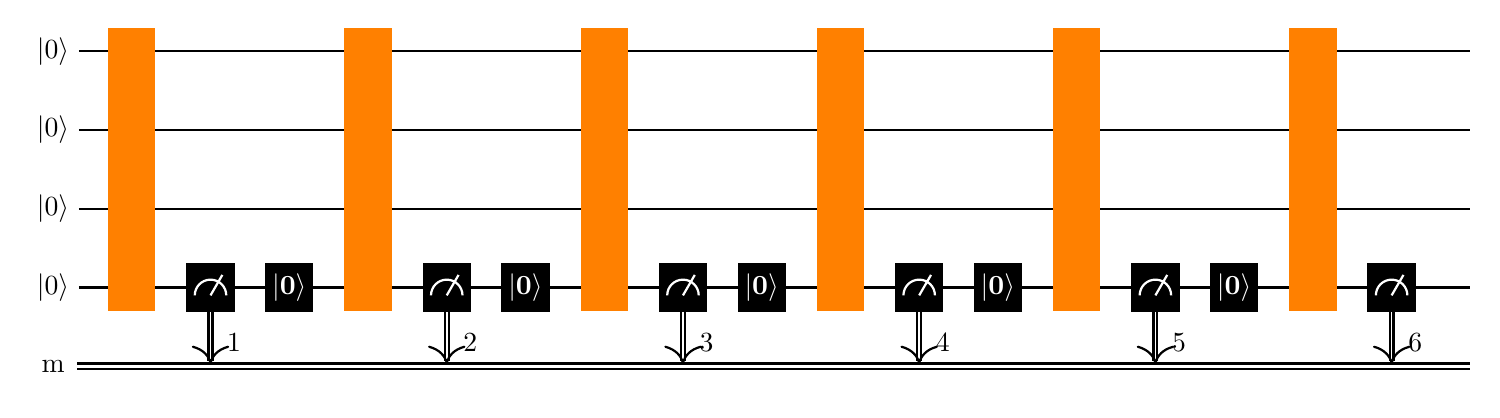
\begin{tikzpicture}[%
		measure/.pic={
			% \draw (-3mm,0) to [bend left] (0,0) to [bend left] (3mm,0);
			\draw[fill=black] (-3mm,-3mm) rectangle (3mm,3mm) ;
			\draw[color=white,thick] (0,-1mm) -- ([yshift=-1mm] 60:3mm)
			 (2mm,-1mm) arc [start angle=0, end angle=180, radius=2mm];
		},
		qubitreset/.pic={
			\draw[fill=black] (-3mm,-3mm) rectangle (3mm,3mm) ;
			\node[color=white] at (0,0) {$\mathbf{\ket{0}}$} ;
		}
		]
	\foreach \q/\i in {q1/1,q2/2,q3/3,q4/4}
	{
		\node[minimum size=6mm] (\q) at (0,\i) {$\ket{0}$};
		\draw[thick] (\q) -- (18,\i) ;
	}
	\node[minimum size=6mm] (m) at (0,0) {m};
	\draw[thick] ($ (m.east) + (0,1pt)$) -- (18,1pt) ;
	\draw[thick] ($ (m.east) + (0,-1pt)$) -- (18,-1pt) ;
	\foreach \i in {0,...,5}
	{
		\path[fill=orange]  ($ (1+3*\i,1) - (0.3,0.3) $) rectangle ($ (1+3*\i,4) + (0.3,0.3) $);
		\draw[thick,double,->] (2+3*\i,1) -- (2+3*\i,1pt) ;
		\node[node font=scriptsize] at (2.3+3*\i,.3) {\the\numexpr\i+1};
		\draw (2+3*\i,1) pic {measure};
		\ifnum\i<5
			\draw (3+3*\i,1) pic {qubitreset};
		\fi
	}
	% \draw[fill=blue] (0.7,5.7) rectangle (1.3,9.3);
\end{tikzpicture}
\end{document}
